The instrument supports three arpeggiator modes.

\scalebox{0.4}{
  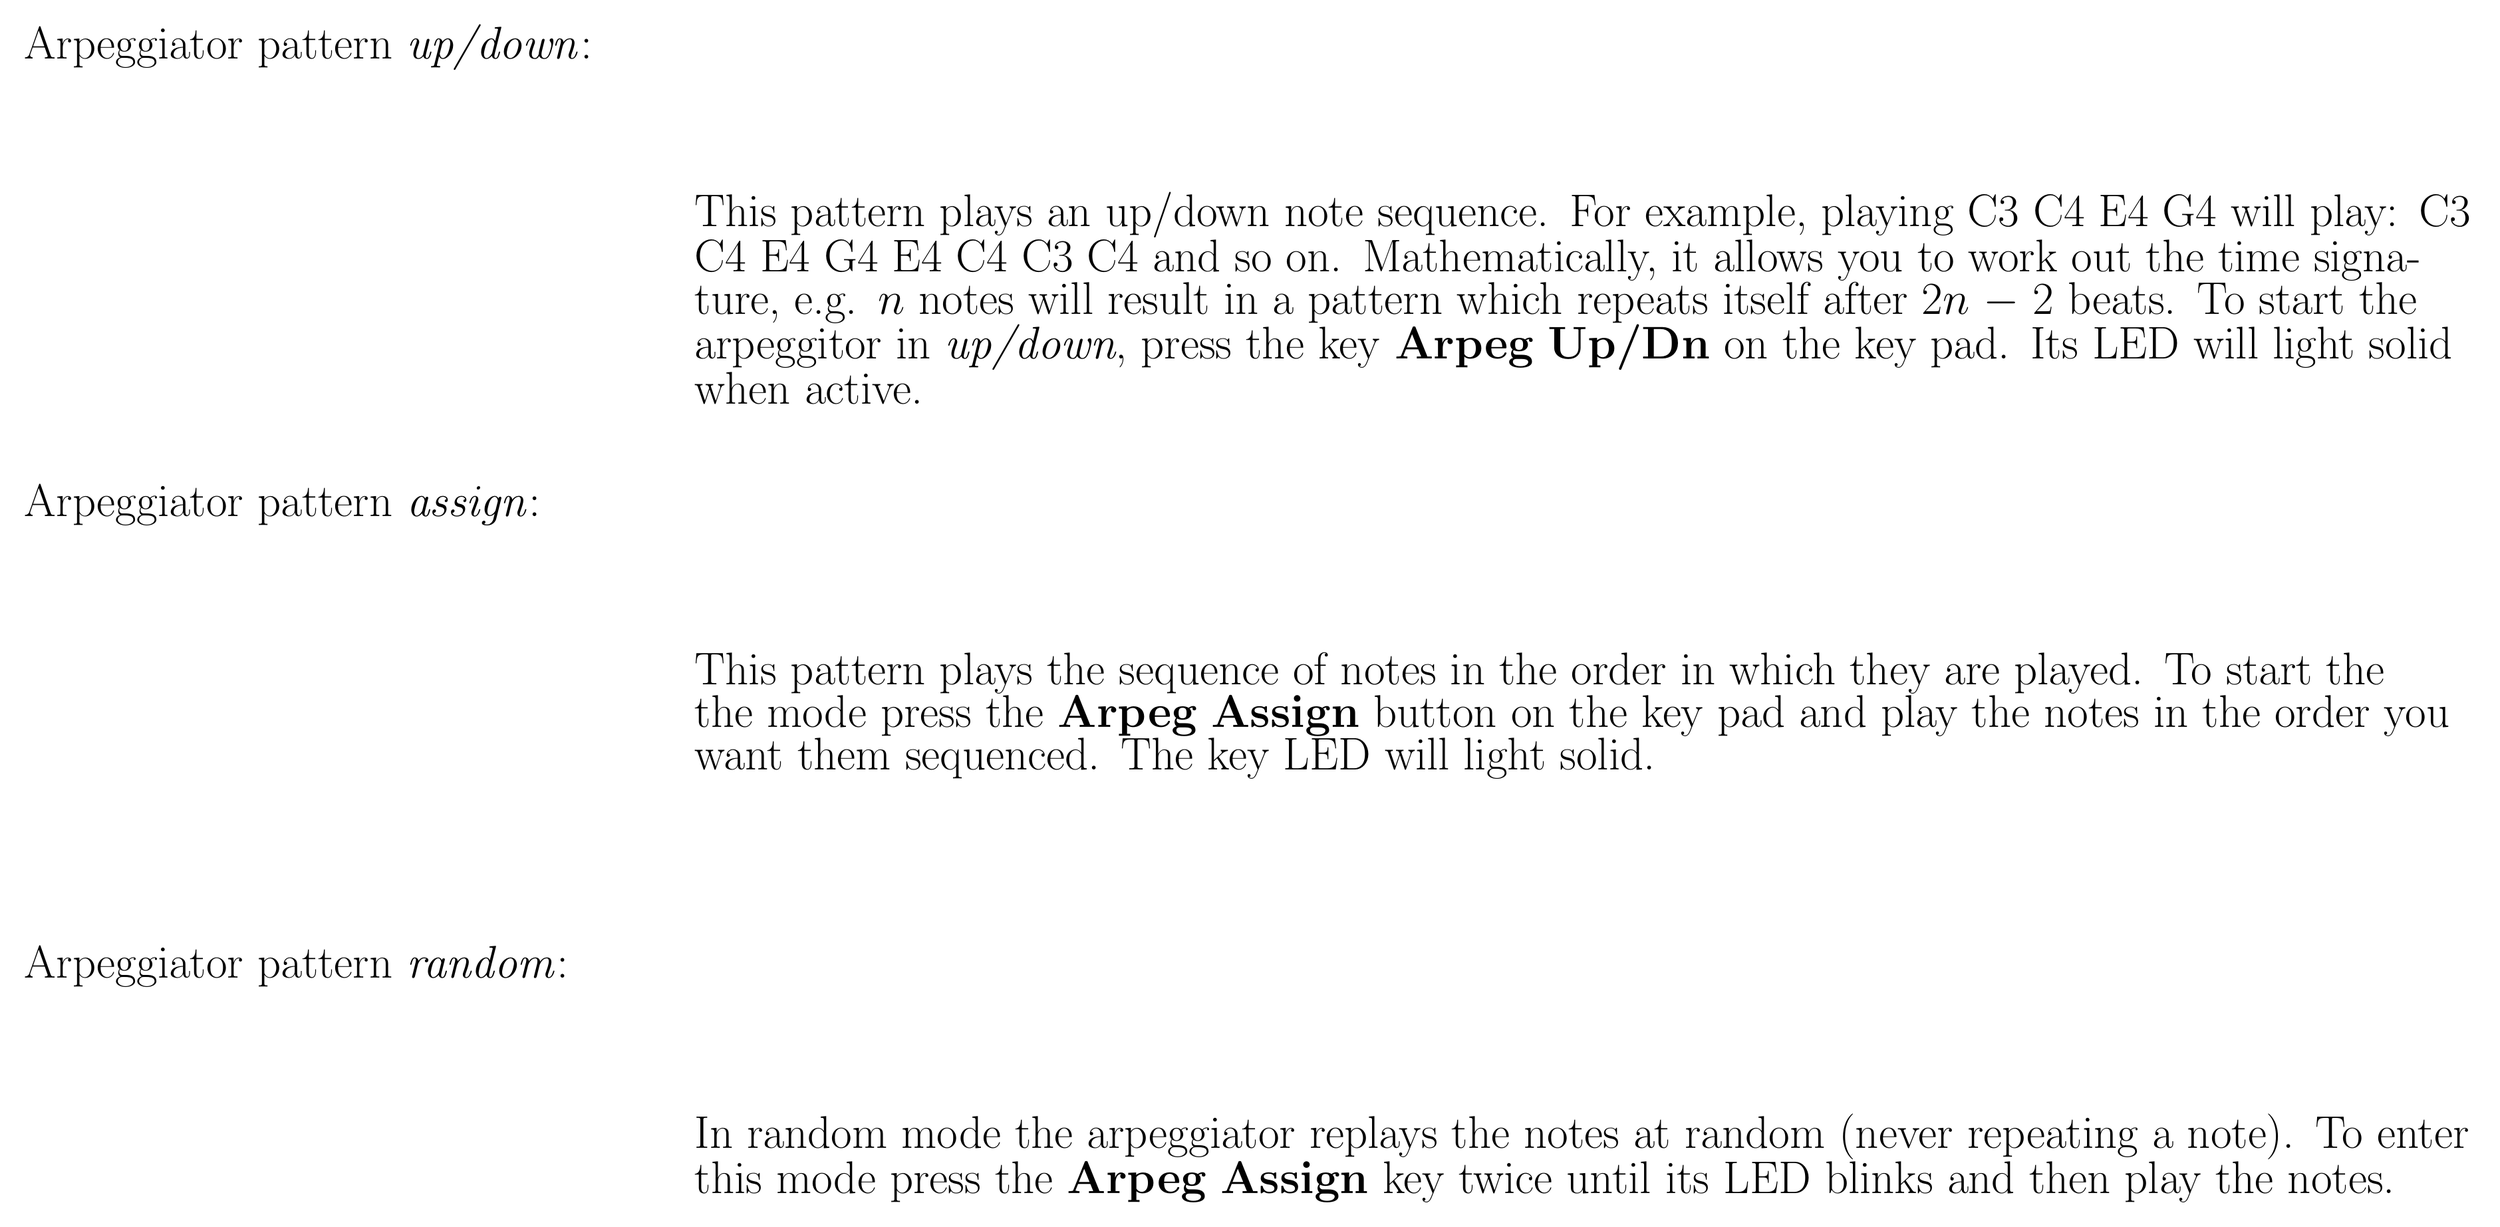
\begin{tikzpicture}[scale=0.8]
  \node[font=\fontsize{26}{22}\selectfont, align=left, outer sep=0.5mm, anchor = north west, text width=30cm] at (0cm,31cm) {Arpeggiator pattern \textit{up/down}:};
  \node[font=\fontsize{26}{22}\selectfont, align=left, outer sep=0.5mm, anchor = north west, text width=34cm] at (16cm,27cm) {This pattern plays an up/down note sequence. For example, playing C3 C4 E4 G4 will play: C3 C4 E4 G4 E4 C4 C3 C4 and so on. Mathematically, it allows you to work out the time signature, e.g. $n$ notes will result in a pattern which repeats itself after $2n-2$ beats. To start the arpeggitor in \textit{up/down}, press the key \textbf{Arpeg Up/Dn} on the key pad. Its LED will light solid when active.};
    \arpsqbuttons{1cm, 22cm}{U}{}
    
  \node[font=\fontsize{26}{22}\selectfont, align=left, outer sep=0.5mm, anchor = north west, text width=30cm] at (0cm,20cm) {Arpeggiator pattern \textit{assign}:};
  \node[font=\fontsize{26}{22}\selectfont, align=left, outer sep=0.5mm, anchor = north west, text width=34cm] at (16cm,16cm) {This pattern plays the sequence of notes in the order in which they are played. To start the the mode press the \textbf{Arpeg Assign} button on the key pad and play the notes in the order you want them sequenced. The key LED will light solid.};
    \arpsqbuttons{1cm, 11cm}{A}{}

    
  \node[font=\fontsize{26}{22}\selectfont, align=left, outer sep=0.5mm, anchor = north west, text width=30cm] at (0cm,9cm) {Arpeggiator pattern \textit{random}:};
  \node[font=\fontsize{26}{22}\selectfont, align=left, outer sep=0.5mm, anchor = north west, text width=34cm] at (16cm,5cm) {In random  mode the arpeggiator replays the notes at random (never repeating a note). To enter this mode press the \textbf{Arpeg Assign} key twice until its LED blinks and then play the notes.};
    \arpsqbuttons{1cm, 0cm}{A}{A}
  \end{tikzpicture}
}


The foot switch input can be used to hold the arpeggiator. Notes send to the Prophet 600 via MIDI are not added to the arpeggiator. It is possible to sync the LFO to the arpeggiator using the additional patch parameter \textbf{(111) LFO Sync}, see section \ref{lfo}.

\textbf{Latch mode}

With all arpeggiator modes, press the \textbf{Record} on the key pad to enter the latch mode where played notes are held. The LED of the button will light solid. Playing additional notes in this mode will add them as additional notes to the existing sequence, up to a maximum of 128 notes. To clear the notes from the sequence, press the Record key to switch it off. The LED of the Record button will go off.

Note that while the random pattern never plays a held note twice in succession. However, since a note can be latched more than once it is possible to 

\textbf{Transpostion}

The arpeggiator pattern can be transposed on the fly. To do so use the keyboard in shifted or shift-locked mode, see section \ref{transposition}.

\textbf{Controlling the arpeggiator using MIDI}

(this needs to be done)


\textbf{Trouble shooting}

If the arpeggiator is activated and keys are held down or have been latched and still no sound plays, then it is worth checking the following potential reasons: Is the sync set to \textit{internal} and is the speed greater than zero (see settings in \ref{settingsref})? If the sync is not \textit{internal} does the instrument receive a clock, e.g. via MIDI on the correct channel or via tape in?
